\chapter{FUNDAMENTAÇÃO TEÓRICA}
\label{FundamentacaoTeorica}

\section{Ambiente de Programação para a \textit{Web}}
\label{AmbienteWeb}

\subsection{\textit{Web}}
\label{SubWeb}

Com o aparecimento da Internet, o significado de \textit{Web} deixou de representar apenas uma rede interligando pontos e ganhou um outro sentido. A \textit{Web} passou a designar uma rede capaz de conectar computadores e pessoas em todo lugar, passando a ser mundialmente conhecida como a \textit{World Wide Web} (WWW). Ou seja, a \textit{Web} significa um sistema de informações ligadas através de hipermídia (hiperligações em forma de texto, vídeo, som e outras animações digitais) que permitem ao usuário acessar uma infinidade de conteúdo por meio da Internet. Estes conteúdos são estruturados através de uma linguagem de marcação como o \textit{HyperText Markup Language} (HTML), personalizados com uma linguagem de estilização \textit{Cascading Style Sheets} (CSS), que podem se tornar dinâmicos com uma linguagem de programação em execução no \textit{Front-End} (i.e. executados no lado cliente), como JavaScript (JS). Após tal processo, o conteúdo pode ser interpretado por um navegador (\textit{browser}) onde são visualizados os conteúdos disponíveis. Desta forma, as páginas podem apresentar informação em diferentes mídias, bem como estarem associadas a dados de estilo ou disponibilizarem funcionalidades interativas ou não. Dentre os diversos navegadores, podem ser destacados os seguintes: Mozilla Firefox, Brave, Opera, Vivaldi, Internet Explorer, Google Chrome, Safari e etc.

O processo de desenvolvimento da \textit{Web} se iniciou em 1980 quando um projeto proposto pela Organização Europeia para a Investigação Nuclear (CERN), chamado de ENQUIRE, foi criado com o intuito de armazenar e reconhecer associações de informações em documentos. Neste projeto, cada documento existente deveria ligar-se a um novo documento. Como resultado, Tim Berners-Lee, funcionário do CERN e inventor do ENQUIRE em 1989, redigiu uma proposta de criação de um grande banco de dados com hiperligações entre documentos. Ou seja, foi apresentada uma solução para resolver o problema de apresentação de informações quando cientistas de várias partes do mundo necessitavam compartilhar dados utilizando diferentes plataformas.

\begin{quote}
\small{
"Em Agosto de 1984 escrevi um artigo ao Chefe do Grupo SW (do CERN), Les Robertson, para descrever um projeto piloto a fim de instalar e avaliar o protocolo TCP/IP em algumas máquinas não Unix do CERN [...] Cerca de 1990, o CERN tinha se tornado o maior sítio da Internet da Europa [...] e do mundo. Um resultado chave de todos estes fatos foi que em cerca de 1989 a rede Internet do CERN estava a tornar-se a medida a partir da qual Tim Berners-Lee viria a criar a \textit{World Wide Web} como uma ideia verdadeiramente ideal..."~\citeonline{segal1995}
}
\end{quote}

Tim Berners-Lee também foi o criador das ferramentas necessárias para o pleno funcionamento da \textit{Web}. Ele desenvolveu o Protocolo de Transferência de Hipertexto (HTTP), a Linguagem de marcação de hipertextos (HTML), além do primeiro navegador e servidor \textit{Web}. Toda a descrição do projeto foi escrita por ele e divulgada na \textit{Web}~\cite{bernerslee1992}.  Atualmente, o projeto encontra-se disponível no sítio oficial da \textit{World Wide Web Consortium} (W3C).

A partir daí, a \textit{Web} tem evoluído constantemente. No momento de sua criação, a expectativa foi de apenas publicação de documentos (i.e. publicação de conteúdo sem interação). Ou seja, ela serviria apenas para informar e trocar informação estática, onde o usuário apenas leria e não haveria interação com os elementos da página. Com o passar dos anos, mais especificamente em 2002, surge o conceito de \textit{Web} 2.0 onde o usuário tem um papel fundamental na criação e personalização do conteúdo. Nesta vertente da interatividade, os blogs foram bastante difundidos, pois a interação do usuário em poder comentar e gerar conteúdo ajudou na expansão exponencial do volume de dados que hoje trafegam na rede. Já na terceira geração da \textit{Web}, ou \textit{Web} 3.0, o foco está para as aplicações \textit{Web}, bem como para o uso da computação gráfica, semântica e inteligência artificial. Portanto, é possível observar um crescimento na publicidade onde o conteúdo exibido para o usuário é personalizado com base nos seus interesses. Ou seja, é uma versão mais inteligente do proposto inicialmente na \textit{Web} 1.0, onde não havia preocupação semântica e visual com as páginas, recursos bastante explorados nas próximas versões.
%
%
%
\subsection{Protocolo HTTP}
\label{SubHTTP}

Como apresentado, o \textit{Hypertext Transfer Protocol} (HTTP) foi um dos primeiros protocolos a serem propostos para o modelo WWW. Ele é o protocolo de transferência de hipertexto adotado em toda \textit{Web} e definido nos \textit{Request for Comments} (RFC) de número 1945 e 2616, \cite{rfc1945} e \cite{rfc2616} respectivamente. O protocolo está implementado na camada de Aplicação da Internet e é responsável pelo funcionamento da \textit{Web}. Este protocolo foi desenvolvido com uma arquitetura cliente-servidor, onde toda a comunicação é realizada através de requisições. O cliente abre uma conexão com o servidor HTTP através do TCP e envia uma requisição (\textit{request}) de conteúdo, que é prontamente retornado por meio de uma resposta (\textit{response}) para o cliente.

\begin{figure}[th]
\centering{
\caption{Requisição HTTP.}
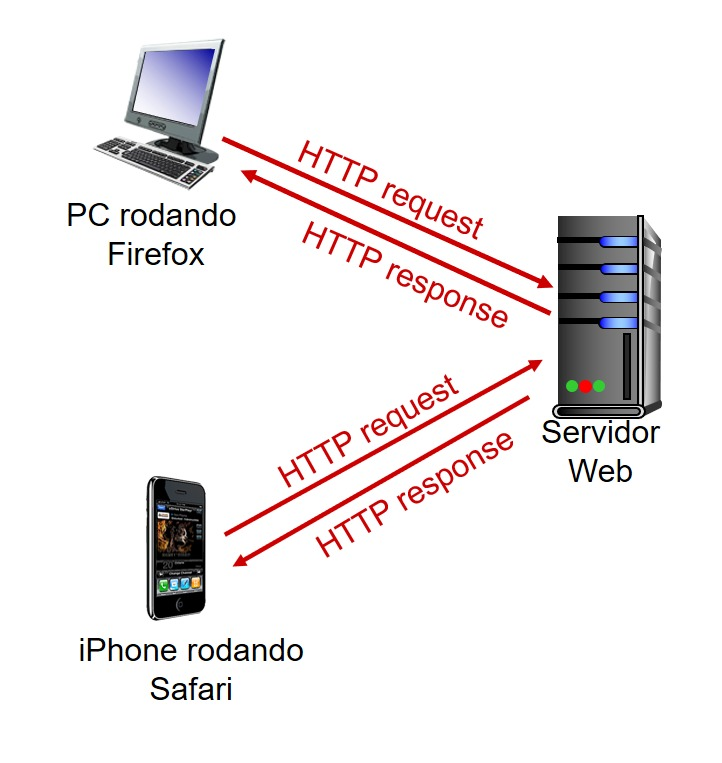
\includegraphics[width=0.5\textwidth]{figuras/reqreshttp}
\begin{flushleft}
\flushleft{Fonte: \citeonline{kurose7th} }
\end{flushleft}
\label{fig:reqreshttp}
}
\end{figure}

Como observado na (Figura~\ref{fig:reqreshttp}), é possível perceber dois clientes se conectando a um único servidor. Cada dispositivo utiliza um navegador diferente em sistemas operacionais e arquiteturas distintas, porém, realizando a requisição HTTP (\textit{request}) e obtendo uma pronta resposta (\textit{response}) do Servidor \textit{Web} em ambas as requisições. O protocolo HTTP funciona independentemente de plataforma, já que, como citado no parágrafo anterior, ele é implementado na camada de Aplicação.

Em cada requisição enviada de um cliente para um servidor, são enviadas também informações detalhadas sobre a requisição, podendo estas irem junto ao corpo (\textit{body}) ou cabeçalho (\textit{header}) da requisição. Podem ser informações sobre o tipo de dado a ser retornado, idioma da resposta ou filtros de dados. Além disso, é passado também um verbo (\textit{HTTP Verb}), que é padrão do protocolo HTTP e define uma série de métodos de requisição responsáveis por indicar a ação a ser executada na representação de um determinado recurso. Cada um deles implementa uma diferente função sendo que alguns recursos são comuns entre todos os verbos. Por exemplo, qualquer método de requisição pode ser do tipo  \textit{safe}, \textit{idempotent}, ou \textit{cacheable}. Abaixo pode-se observar a lista completa de verbos existentes como também seus detalhamentos:
\begin{itemize}
    \item \textbf{GET}~\textemdash~esse método é utilizado para solicitar uma representação de um recurso específico, Requisições utilizando o Método GET devem retornar apenas dados;
    \item \textbf{HEAD}~\textemdash~solicita uma resposta de forma idêntica ao processo que ocorre no tipo GET, porém sem um corpo \textit{body} contendo o recurso;
    \item \textbf{POST}~\textemdash~utilizado para submeter uma entidade a um recurso específico, às vezes causando uma mudança no estado do recurso ou solicitando alterações do lado do servidor;
    \item \textbf{PUT}~\textemdash~substitui todas as atuais representações de seu recurso alvo pela carga de dados da requisição;
    \item \textbf{DELETE}~\textemdash~remove um recurso específico;
    \item \textbf{CONNECT}~\textemdash~estabelece um túnel para conexão com o servidor a partir do recurso alvo;
    \item \textbf{OPTIONS}~\textemdash~usado para descrever as opções de comunicação com o recurso alvo;
    \item \textbf{TRACE}~\textemdash~executa uma chamada de loopback como teste durante o caminho de conexão com o recurso alvo;
    \item \textbf{PATCH}~\textemdash~utilizado para aplicar modificações parciais em um recurso.
\end{itemize}

Atualmente, o protocolo HTTP está passando por uma evolução, saindo da versão 1.1 para o HTTP/2 padronizado no RFC 7540 (\cite{rfc7540}). Em sua mais nova versão, pode-se observar um ganho de performance, visto que ele não é mais um protocolo criado para ser entendido por humanos, mas lido por máquinas. Por esse motivo, é mais eficiente e traz alguns benefícios que consertam os problemas atuais da \textit{Web}. Otimizado, o HTTP/2 usa multiplexação, um nome complicado para dizer que o navegador abre uma única conexão para baixar múltiplos arquivos. Desta forma, as requisições e respostas são paralelas e assíncronas, ou seja, o seu navegador pede vários arquivos ao mesmo tempo e recebe-os assim que eles estiverem prontos, na mesma conexão. Já no HTTP/1.1 (RFC 2616 e versão mais utilizada atualmente) o navegador abre uma conexão para baixar um único arquivo. Se essa conexão ficar ocupada por muito tempo, seja porque o arquivo é muito grande ou porque o servidor está lento para responder, o carregamento da página simplesmente trava no meio do processo. Há como amenizar esse problema abrindo múltiplas conexões, mas isso é apenas uma solução paliativa e, não uma solução permanente. Este trabalho, entretanto, está direcionado a transmitir apenas boas práticas de programação e dicas de otimização de código e performance, evitando soluções paliativas.
%
%
%
\subsection{Navegador}
\label{SubNavegador}

Responsável por toda interação visual do lado cliente (i.e. arquitetura \textit{client-server}), o \textit{browser} ou navegador é quem renderiza as páginas \textit{Web}. Além disso, o navegador trata o DOM (\textit{Document Object Model}), realiza requisições e cuida dos eventos de interação do usuário. Ou seja, sem o navegador, a Internet não teria se desenvolvido tanto quanto vem crescendo nos últimos anos. Isso porque ele deixa tudo mais fácil e intuitivo. Dentre as várias partes de um navegador moderno e funcional, devem ser citado e destacado o motor de renderização, também chamado de mecanismo de renderização, que é quem transforma linguagem de marcação (i.e. HTML, XML, etc.) e informações de formatação (i.e. CSS, XSL, etc.) em um conteúdo formatado para ser exibido em uma tela.

De acordo com o Decálogo da \textit{Web}, definido pelo W3C, qualquer pessoa tem o direito de acessar a informação de forma igualitária. Não importa se o acesso de determinado site é realizado via \textit{tablet}, \textit{desktop}, \textit{smartphone} ou até mesmo a partir de uma TV. Todos têm direito de acessar todas as informações como se estivessem em um \textit{desktop} de última geração. Ainda de acordo com a documentação da W3C, cada um destes meios de acesso utilizam um determinado \textit{browser} para navegar na \textit{Web}.

Todo \textit{browser} carrega apenas um motor de renderização, para o usuário que apenas faz uso do mesmo ao navegar pela \textit{Web}, o processo de faz de forma transparente. No entanto, existem diversos mecanismos de renderização e cada um funciona de maneira distinta para cada dispositivo/equipamento, podendo haver semelhanças ou incompatibilidades entre um e outro. Para o desenvolvedor que é quem constrói um sistema \textit{Web}, não é viável desenvolver um sistema exclusivamente para determinado motor (\textit{engine}). Para tal, a W3C provê uma documentação única e os motores de renderização implementam suas funcionalidades com base nesta documentação a fim de se obter uma padronização ou, no mínimo, um resultado visual eficiente. Portanto, o desenvolvedor precisa apenas utilizar as boas práticas para obter o máximo de produtividade possível e diminuir a quantidade de conflitos por incompatibilidade entre \textit{engines}. Atualmente os dois motores mais utilizados são o \textit{Webkit} e \textit{Gecko} que correspondem aos navegadores: Opera, Safari, Google Chrome, Vivaldi e Brave (\textit{Webkit}, porém, portando para o \textit{Blink}); Mozilla Firefox (\textit{Gecko}, porém, portando para o \textit{Servo}); Além do Internet Explorer (\textit{Spartan}).

Além da renderização o navegador também contém um interpretador JavaScript, também chamado de motor JavaScript, que é um \textit{software} especializado que interpreta e executa JavaScript ou ECMAScript. Assim como os motores de renderização, também existem diversos interpretadores JavaScript. Dentre eles, os mais impactantes são:
\begin{itemize}
    \item \textit{SpiderMonkey}~\textemdash~O primeiro interpretador, criado por Brendan Eich, criador do JavaScript, para o Netscape;
    \item \textit{Squirrelfish Extreme}~\textemdash~Desenvolvido para \textit{Webkit} e desenvolvido pela Google;
    \item \textit{TraceMonkey}~\textemdash~Desenvolvido exclusivamente para o Mozilla Firefox e mais veloz que o concorrente \textit{Webkit};
    \item \textit{V8}~\textemdash~Réplica da Google, uma nova tentativa de se tornar o melhor navegador com o Chrome 2.0. Atual \textit{engine} do navegador.
\end{itemize}

Pode-se observar que há uma disputa por velocidade e otimização entre todos os motores de renderização, interpretadores e afins. Tudo por uma \textit{Web} mais veloz e cada vez mais padronizada (\textit{Web Standards}). A cada dia, novas versões, novos motores e até linguagens surgem para tornar mais veloz a navegação. No momento em que este trabalho foi escrito, destaca-se a existência de implementações do \textit{Web Assembly}, porém, infelizmente, ainda não há versão estável. Portanto, estas implementações não serão citadas neste guia para o desenvolvimento de aplicações \textit{Web}.

\begin{figure}[th]
\centering{
\caption{Árvore DOM.}
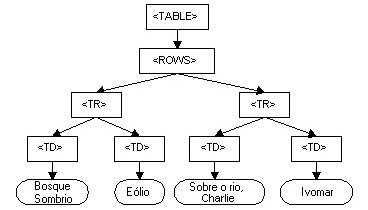
\includegraphics[width=0.5\textwidth]{figuras/domtree}
\begin{flushleft}
\flushleft{Fonte: Retirado de \citeonline{wood2004document} }
\end{flushleft}
\label{fig:domtree}
}
\end{figure}

Não pode-se esquecer do DOM, criado pelo W3C, que é uma multi-plataforma que representa como as marcações em HTML, XHTML e XML são organizadas e lidas pelo navegador. Uma vez indexadas, estas marcações se transformam em elementos de uma árvore que podem ser manipuladas via API. Em outras palavras, pode-se utilizar o DOM para alterar funcionalidades de uma página, tais como o conteúdo, a estrutura ou o estilo.

A (Figura~\ref{fig:domtree}) apresenta a representação gráfica de uma árvore DOM após a leitura de uma tabela HTML. Como percebe-se, o DOM é a base para uma outra árvore que é o que realmente um \textit{browser} monta na tela, a Árvore de Renderização (\textit{Render Tree}). A base para todos os nós da árvore DOM é a classe base chamada \textbf{Node.h}. Ela possui várias categorias, e as relevantes para renderizar código no navegador são os nós de documentos, elementos e texto.
\begin{itemize}
    \item \textbf{Documentos} é o nó mais importante do DOM, com três classes diferentes: \textit{Document}, que é usado por todos os documentos XML e outros que não sejam SVG (que também é um XML, porém com marcação já padronizada), \textit{HTMLDocument} que como o nome diz, cuida de documentos HTML e \textit{SVGDocument}, responsável pelos documentos SVG e também por outros documentos herdados da classe \textit{Document} (Como o \texttt{Document.h} e o \texttt{HTMLDocument.h}).
    \item \textbf{Elementos} são todas as \textit{tags} que estão em arquivos HTML ou XML se transformam em elementos da árvore DOM. Considerando a renderização do navegador, um elemento é um nó com uma \textit{tag} que pode ser usada para fazer subclasses específicas, que podem ser processadas de acordo com as necessidades da árvore de renderização (\texttt{Element.h}).
    \item \textbf{Texto} é propriamente o texto que vai entre os elementos. Todo o conteúdo das \textit{tags}.
\end{itemize}
%
%
%
%
%
%
%
%
%
\section{Tecnologias Básicas de uma Aplicação \textit{Web}}
\label{BaseWeb}

%Quando se estuda sobre Aplicações \textit{Web}, é muito comum se deparar com comparações entre as tecnologias e o mundo real. A mais famosa no contexto de HTML, CSS e JS é:
\begin{quote}
\small{
"HTML é como o pai engenheiro, ele é responsável por estruturar as coisas, garantir que haja um sólido. CSS se parece com a mãe arquiteta, ela embeleza a estrutura, dá brilho e glamour para a criação e fornece o apreço visual pela obra. Já o JS é o filho nerd que brinca com o \textit{Arduino} pela casa, ele faz tudo funcionar, é ele quem faz a mágica acontecer".~Fábio Magnoni.
}
\end{quote}

\subsection{HTML}
\label{SubHTML}

HTML é a sigla em inglês para \textit{HyperText Markup Language}, que, em português significa linguagem para marcação de hipertexto~\footnote{Hipertexto é uma referência aos \textit{links} que interligam páginas, independente se estão localizadas localmente (i.e. mesmo \textit{Website}) ou externamente.}. O HTML é o construtor de blocos mais básico da \textit{Web}. Ela serve para descrever e definir o conteúdo de um documento. Desde a invenção da \textit{Web} por Tim Berners-Lee, a linguagem HTML evoluiu por oito versões, que são: HTML; HTML +; HTML 2.0; HTML 3.0; HTML 3.2; HTML 4.0; HTML 4.01; HTML 5~\footnote{A WHATWG trabalha na versão do HTML5 (observe os espaços), enquanto a W3C se baseia no HTML5 para documentar o HTML 5} (versão atual).

Oficialmente, a W3C, principal organização de padronização da \textit{World Wide Web}, considera apenas 5 versões. Isso deve-se ao fato de duas terem sido criadas antes mesmo da W3C, além do HTML 3.0, nunca lançado oficialmente.

\begin{quote}
\small{
"Tim Berners-Lee acreditava que seria possível interligar hipertextos em computadores diferentes com o uso de links globais, também chamados de hiperlinks. Ele desenvolveu um software próprio e um protocolo para recuperar hipertextos, denominado HTTP. O formato de texto que criou para o HTTP foi chamado de HTML. Tim tomou como base para a criação da HTML a especificação SGML, que é um método internacionalmente reconhecido e aceito, contendo normas gerais para a criação de linguagens de marcação."~\citeonline{html5majour}
}
\end{quote}

Desde sua criação, em 1991, a HTML tem evoluído bastante tanto em sua especificação quanto em seus recursos e escrita. Entretanto, desde o início, ela utiliza marcação (\textit{markup}) para envolver os conteúdos renderizados pelo navegador, tais como textos, imagens e miscelânea. A base do funcionamento está diretamente ligada às \textit{tags} ou etiquetas e também aos atributos. No trecho de Código~\ref{htmlbase}, é importante observar a estrutura básica de um arquivo HTML, chamado de \texttt{index.html}
\begin{lstlisting}[label=htmlbase,caption=Estrutura Básica de um código HTML.]
<!DOCTYPE html>
<html lang="pt-br">
    <head>
        <meta charset="utf-8">
        <title>Monografia</title>
    </head>
    <body>
        <h1>Aqui escrevo minha monografia</h1>
        
        <p>Em <strong>2008</strong> conheci a HTML.</p>
    </body>
</html>
<!-- Salve engano -->

\end{lstlisting}

Após uma breve observação do código, segue abaixo a explicação detalhada de sua estrutura básica:
\begin{itemize}
    \item \textbf{Linha 1}: É declarado o tipo do documento em questão, no caso um arquivo HTML.
    \item \textbf{Linha 2}: É iniciada/aberta a \textit{tag} principal. Logo após, há um atributo chamado \textit{lang} que informa o idioma deste documento HTML.
    \item \textbf{Linhas 3 a 6}: Este é o cabeçalho da página e dentro dele estão contidas informações referentes à página, como codificação e título do documento.
    \item \textbf{Linhas 7 a 11}: Chegamos ao corpo do documento, onde o conteúdo está disponível.
    \item \textbf{Linha 8}: Um elemento de título foi criado e um texto foi inserido dentro deste elemento.
    \item \textbf{Linha 10}: Um elemento de texto \texttt{<p>} é criado, ele é um parágrafo. Seu conteúdo tem um texto simples e um destaque dentro de um elemento \texttt{<strong>} que, por padrão, deixa a fonte em negrito.
    \item \textbf{Linha 12}: Finalização/Fechamento da \textit{tag} principal e fim do código.
    \item \textbf{Linha 13}: Exemplo de comentário.
    \item \textbf{Linha 14}: Apesar de não ser visível, EOF ou Fim do Arquivo, é comum em ambientes UNIX a existência de uma linha em branco em arquivos não vazios. Esta é uma boa prática de desenvolvimento que é adotada neste trabalho.
\end{itemize}

O Resultado do Código~\ref{htmlbase} pode ser observado na Figura~\ref{fig:htmlbase}.

\begin{figure}[th]
\centering{
\caption{Exemplo de Código HTML.}
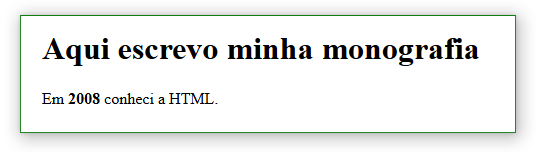
\includegraphics[width=0.5\textwidth]{figuras/htmlbase}
\begin{flushleft}
\flushleft{Fonte: Elaborado pelo autor.}
\end{flushleft}
\label{fig:htmlbase}
}
\end{figure}

É natural delimitar o fechamento de uma \textit{tag} com uma barra~"\texttt{/}"~seguido do restante do nome da \textit{tag} aberta. Elementos desta natureza são chamados de elementos de bloco. Há também os elementos vazios que não necessitam de fechamento de \textit{tag}. No exemplo do Código~\ref{htmlbase}, pode-se perceber a \textit{tag}~\texttt{<meta>}.

Para fins nominais, a terminologia prevê, no exemplo da Linha 10 do Código~\ref{htmlbase}, que há em \texttt{<p>} uma Abertura de \textit{Tag} e em \texttt{</p>} seu fechamento. O que está entre as duas \textit{tags} deste elemento em bloco \texttt{<p>} é o conteúdo, e todo o conjunto se denomina Elemento. Elementos podem conter atributos, que são declarados logo após a abertura da \textit{tag} e separados por um espaçamento. Além disso, os atributos podem ser múltiplos ou inexistentes dentro de um elemento e possuem o padrão de Chave-Valor, onde a chave é declarada inicialmente, seguido por um sinal de igualdade, e o valor é declarado dentro de aspas duplas~\texttt{"valor"}. Ainda na mesma linha 10, observa-se um exemplo de Aninhamento, que é o fenômeno que ocorre quando um elemento é declarado dentro de outro elemento.

A HTML traz para as suas \textit{tags} uma tipografia \textit{case insensitive} (i.e. não diferencia caracteres maiúsculos e minúsculos), ou seja, é possível declarar \texttt{<section>} ou \texttt{<SECTION>} ou até mesmo \texttt{<SeCtIoN>}. No entanto, para garantir um código limpo e fácil de ler e entender por toda a equipe de desenvolvimento, recomenda-se como uma boa prática de desenvolvimento, manter o nome da \textit{tag} em letras minúsculas (ex.: \texttt{<section>}). Adicionalmente, caso um dia seja necessário declarar um elemento com nome composto, a recomendação é utilizar o hífen para separar o nome do elemento, ou seja, declara-se \texttt{MeuElemento} como \texttt{<meu-elemento>}.

É possível aprender HTML de uma maneira muito fácil, pois há diversas fontes de conteúdo na Internet. A fonte mais completa e constantemente atualizada é o diretório HTML em \textit{\citeonline{mdn}}, mantida pela comunidade ativa da Mozilla.
%
%
%
\subsection{CSS}
\label{SubCSS}

CSS (\textit{Cascading Style Sheets}) ou folhas de estilos em cascata é uma linguagem de estilo utilizada para personalizar a apresentação de um documentos \textit{Web}, ou seja, CSS é um padrão de formatação (\textit{Web Standards~\footnote{\textit{Web Standards} é um conjunto de normas, diretrizes, recomendações, notas, artigos, tutoriais e afins de caráter técnico, e destinados a orientar fabricantes, desenvolvedores e projetistas para o uso de práticas que possibilitem a criação de uma \textit{Web} acessível a todos, independentemente dos dispositivos usados ou de suas necessidades especiais.}}) para páginas que permite ir além das limitações impostas pela HTML. Quando se deseja garantir uma formatação homogênea e uniforme em todas as páginas de um site as folhas de estilo em cascata facilitam muito o trabalho de criação.

Quando a HTML foi finalmente implementada, o esforço não foi de maneira alguma, formatar os dados, mas exibir o que previamente foi marcado com as \textit{tags} conhecidas na Subseção~\ref{SubHTML}. Com a popularização da HTML, houve a necessidade de implementar atributos de estilo para alterar algumas aparências da página. Isto fez com que o código ficasse muito complexo e difícil para se manter, visto que tudo estava misturado. Outro fator a se destacar foi a falta de padronização nas implementações dos navegadores daquela época, o que dificultava a visualização das páginas, exibindo conteúdos visualmente distintos entre \textit{browsers}. Estes problemas infelizmente ainda acontecem, porém, pode ser minimizado com boas práticas, como separar o código HTML do CSS e utilizar abordagens mais genéricas e/ou bibliotecas CSS previamente testadas pela comunidade ativa de desenvolvedores. Isso permite evitar o retrabalho por parte do programador, pois o mesmo pode utilizar ferramentas existentes e focar apenas no produto, realizando apenas pequenas intervenções. Tudo isso permite a garantia de uma melhor experiência \textit{cross-browser}~\footnote{\textit{Cross-Browser} refere-se à habilidade de um site suportar múltiplos navegadores sem comprometer o estilo previamente implementado.} e \textit{cross-platform}~\footnote{\textit{Cross-Platform} é a denominação de uma Aplicação \textit{Web} que foi desenvolvida para funcionar independente de plataforma.} para o usuário.

Em 1994, Håkon Wium Lie e Bert Bos propuseram a criação do CSS, após observarem todo este cenário caótico no desenvolvimento de Aplicações \textit{Web}, uma maneira mais fácil de formatar a apresentação da página. Em 1995 a proposta foi apresentada ao \textit{World Wide Web Consortium} (W3C), o qual é uma comissão que define os padrões de programação para a WWW. Recém criada, a W3C demonstrou interesse pelo projeto e montou uma equipe de desenvolvimento que viria a finalizar seu primeiro projeto em 1996. Foi assim que surgiu a primeira versão do CSS. A história do CSS é descrita em mais detalhes no capítulo 20 do livro CSS: Projetando para a \textit{Web}, escrito pelos próprios criadores \citeonline{lie2005cascading}.

Atualmente, o CSS encontra-se em sua versão estável de número 3 (CSS 3) e em desenvolvimento da versão 4 (CSS 4), proposta por~\citeonline{css4}~nos diretórios da W3C. As evoluções do CSS trouxeram mais recursos e aumentaram a sua abrangência, porém, mantendo o mesmo princípio de formatar a aparência das páginas \textit{Web}. Inicialmente, apenas cores eram mudadas. Após isso, o comportamento pode ser manipulado também. Então foi possível definir o tamanho dos elementos apenas com CSS e por fim, temos animações e efeitos em 3D, além de cada vez mais suporte à responsividade~\footnote{Design Responsivo é uma técnica de estruturação HTML e CSS, em que o site se adapta ao browser do usuário sem precisar definir diversas folhas de estilos para cada resolução.}.

É possível inserir regras de estilo em cascata de três formas junto a um documento HTML. São elas:
\begin{itemize}
    \item \textit{Inline}~\textemdash~via atributo HTML, adicionando ao atributo \texttt{style} o seu código CSS. Desta forma, o código inserido refletirá sobre o elemento ao qual a propriedade foi declarada.
    \item \textit{Embedding}~\textemdash~via \textit{tag} \texttt{<style>}. Dentro do cabeçalho (\texttt{<head>}), é possível inserir trechos genéricos de código CSS. Podendo aplicá-los a todo o documento ou apenas a trechos específicos.
    \item \textit{Linking}~\textemdash~utilizando um ou mais arquivos externos de folha de estilo em cascata com a extensão \texttt{.css}, importados dentro do documento HTML.
\end{itemize}

O \textit{Linking} é considerado a melhor prática para se trabalhar com folhas de estilo em cascata, pois, além de ser a maneira mais recomendada, é também a estratégia mais organizada para descentralizar o estilo \textit{inline} dos componentes. Em outras palavras, utilizando o atributo \texttt{<style>}. A vantagem de se utilizar uma importação \textit{Linking} ao invés de \textit{Embedding} se resume pelo fato de reduzir o tamanho de linhas no documento HTML, garantindo uma melhor leitura de código e separação das tecnologias, com o objetivo de facilitar a manutenção de código.

A estrutura de código CSS, assim como HTML é muito fácil de aprender. Juntamente ao arquivo \texttt{index.html} (Código~\ref{htmlbase}), cria-se um outro arquivo chamado \texttt{style.css}, que contém o código CSS (Código~\ref{cssbase}). As regras de estilização podem ser observadas logo abaixo.
\begin{lstlisting}[label=cssbase,caption=Exemplo de um código CSS.]
/* h1 vai ser vermelho */
h1 {
    color: red;
}

/* o paragrafo tera uma borda azul */
p {
    border: 1px solid blue;
}
\end{lstlisting}

Como descrito através dos comentários do código acima, observam-se duas modificações visuais. A primeira é a cor vermelha no elemento de título~"\texttt{<h1>}"~e a segunda está relacionada ao parágrafo com a definição de uma borda na cor azul. Diferente do atributo de cor~"\texttt{color}"~que tem apenas uma propriedade, o atributo de borda~"\texttt{border}"~possui três propriedades, que são: 
\begin{itemize}
    \item \textbf{Tamanho}~\textemdash~O tamanho foi definido em \textit{pixels}, mas existem diversas outras unidades de medida disponíveis no CSS como \texttt{px}, \texttt{rem}, \texttt{rm}, \texttt{em}, \texttt{ch}, \texttt{\%} dentre outras.
    \item \textbf{Estilo}~\textemdash~O tipo da borda escolhido foi a simples. Ou seja, uma borda sólida com a espessura previamente definida através do tamanho. Além disso, poderia ser uma borda pontilhada~"\texttt{dashed}", dupla~"\texttt{double}"~ou outro tipo de borda.
    \item \textbf{Cor}~\textemdash~A cor pode ser definida pelo nome em inglês ou por meio de uma codificação em RGB~"\texttt{rgb(0, 0, 255)}"~ou hexadecimal~"\texttt{\#0000ff}", por exemplo.
\end{itemize}

Todos estes detalhes e valores das propriedades CSS podem ser consultadas no \textit{\citeonline{mdn}} do diretório CSS. 

É importante destacar a estrutura do bloco, inicialmente um seletor é declarado e logo após chaves "\texttt{{ }}" são abertas e o código é inserido dentro delas. É possível perceber a semelhança com os atributos HTML pelo fato de existir um sistema de chave e valor, separados pelos dois pontos "\texttt{:}" e finalizando o comando com ponto e vírgula "\texttt{;}". Apesar deste ser um guia de boas práticas, não são utilizadas classes no código de exemplo. Para utilizar classes na HTML basta atribuir \texttt{class="titulo"} no elemento \texttt{<h1>} e, em seguida, alterar a linha 2 para \texttt{.titulo} no código CSS. O ponto é um identificador de classe~\footnote{O identificador ponto~"\texttt{.}"~a frente do nome do seletor indica uma classe e o identificador cerquilha~"\texttt{\#}"~referencia um identificador único (i.e. \texttt{id="titulo"}).}.

Para garantir o pleno funcionamento e ligar o código de estilo ao arquivo \texttt{index.html}, é necessário importá-lo. Para isso, basta adicionar dentro do cabeçalho do Código~\ref{htmlbase} o trecho de código disponível em~\ref{inserircssnohtml}, que é um elemento de \textit{link}. Desta forma, seus atributos \texttt{rel} e \texttt{type} definem uma folha de estilo do tipo CSS e o atributo \texttt{href} informa o caminho onde está localizado o arquivo \texttt{style.css} em questão. Neste exemplo, o arquivo localiza-se no mesmo diretório do arquivo \texttt{index.html} criado.
\begin{lstlisting}[label=inserircssnohtml,caption=Inserir CSS externo no HTML.]
<link rel="stylesheet" type="text/css" href="style.css" />
\end{lstlisting}

Como resultado das implementações, é possível observar na Figura~\ref{fig:cssbase}, uma página \textit{Web} mais colorida.

\begin{figure}[th]
\centering{
\caption{Exemplo de Código CSS.}
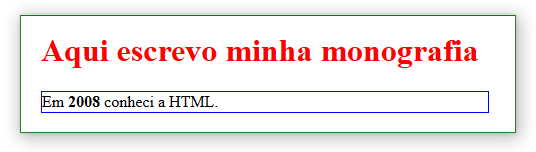
\includegraphics[width=0.5\textwidth]{figuras/cssbase}
\begin{flushleft}
\flushleft{Fonte: Elaborado pelo autor.}
\end{flushleft}
\label{fig:cssbase}
}
\end{figure}

É importante salientar que as boas práticas existem para evitar erros e confusões no desenvolvimento do projeto. Se tratando de CSS, um dos maiores problemas está relacionado à precedência. Em outras palavras, é necessário evitar que duas regras de estilo sejam aplicadas para um mesmo elemento HTML especificado. Por exemplo, se houver diferentes modos de estilo (exemplo: \textit{Inline} e \textit{Linking}) as especificações podem entrar em conflito. Desta forma, o navegador é responsável por intermediar e decidir qual estilo conflitante deverá prevalecer baseado em quem tem maior ordem de precedência. A ordem de precedência adotada pelos navegadores felizmente é padronizada e sua definição é:
\begin{itemize}
    \item \textit{Inline} ou Estilo em linha~\textemdash~dentro de um elemento HTML.
    \item \textit{Embedding} ou Folha de estilo incorporada~\textemdash~definida no cabeçalho do documento.
    \item \textit{Linking} ou Folha de estilo externa~\textemdash~importada e referenciada.
    \item \textit{Default} ou Estilo padrão do navegador~\textemdash~estilo predefinido.
\end{itemize}

É importante lembrar esta ordem de precedência para que se saiba qual valor de estilo tem maior prioridade. Assim sendo, um estilo \textit{inline} tem a prioridade mais elevada, o que significa que prevalece sobre aquele definido no cabeçalho do documento, que, por sua vez, é prioritário em relação ao definido em uma folha de estilo em cascata externa e esse sobre o formato que o navegador especifica~\footnote{É comum utilizar estilos CSS para reiniciar a aparência padrão do navegador, visto que, os navegadores apresentam pré-formatações de estilo distintas. Esta é uma boa prática.}.

Para os estilos \textit{Embedding} e \textit{Linking} onde o código é definido por blocos, há a possibilidade de se tratar a herança além de pseudo-classes~\footnote{Uma pseudo-classe CSS é uma palavra-chave adicionada aos seletores que especifica um estado especial do elemento a ser selecionado.}. Por exemplo, quando o usuário passa o ponteiro do mouse sobre determinado elemento, este evento ou estado especial é chamado de \textit{hover} e pode ser inserido \texttt{:hover} após o seletor CSS (exemplo: \texttt{h1:hover \{}). Isto faz com que o evento de \textit{hover} seja acionado e um estilo, normalmente diferente do inicialmente renderizado, seja aplicado ao elemento que ativou o evento em questão. Existem diversas pseudo-classes que identificam diversos eventos de página, tanto em relação aos eventos causados pela interação do usuário com a aplicação (exemplo: \texttt{:hover}) quanto eventos de estado de elementos (exemplo: \texttt{:disabled}) e até herança (exemplo: \texttt{:first-child}). Portanto, as pseudo-classes para seletores CSS, tem tornado o desenvolvimento muito mais fácil e intuitivo.

\begin{figure}[th]
\centering{
\caption{Modelo de Caixa no CSS.}
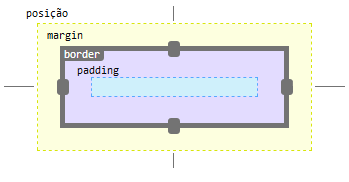
\includegraphics[width=0.5\textwidth]{figuras/boxmodel}
\begin{flushleft}
\flushleft{Fonte: Developer Tools do Mozilla Firefox Nightly (61.0a1).}
\end{flushleft}
\label{fig:boxmodel}
}
\end{figure}

Outros detalhes importantes sobre CSS estão relacionados à orientação das margens (\textit{margin}), preenchimentos (\textit{padding}) e bordas (\textit{border}). Na Figura~\ref{fig:boxmodel}, é possível observar cada uma das orientações. O espaçamento externo ao elemento definido por~\texttt{margin}~e interno definido por~\texttt{padding}, que distancia o conteúdo do elemento das bordas, que, trivialmente é definido por por~\texttt{border}.
%
%
%
\subsection{JavaScript}
\label{SubJS}

JavaScript, ou simplesmente JS, é uma linguagem de programação de alto nível, dinâmica e interpretada do lado cliente (i.e. processada pelo navegador), desenvolvida por Brendan Eich. O JavaScript, juntamente com HTML e CSS é um dos três pilares que atualmente sustentam a rede mundial de computadores (\textit{World Wide Web}). No entanto, o JS é o principal responsável por tornar as páginas da \textit{Web} interativas. Foi originalmente desenvolvido com o nome de Mocha. Posteriormente, teve seu nome modificado para LiveScript e, por fim, JavaScript. LiveScript foi o nome oficial da linguagem quando ela foi lançada pela primeira vez, na versão beta do navegador Netscape 2.0, em setembro de 1995. Entretanto, teve seu nome alterado em um anúncio conjunto com a \textit{Sun Microsystems}, em dezembro do mesmo ano, quando foi implementado no navegador Netscape, versão 2.0B3.

Neste instante, a Netscape percebeu que a WWW precisava se tornar mais dinâmica, com o objetivo de realizar tarefas simples como verificar se os usuários inseriam valores corretos em um formulário. Algo dessa natureza precisaria enviar os dados para um servidor, para que esse interpretasse os dados e retornasse uma saída.

A linguagem é padronizada pela~\citeonline{ecma}, uma associação Europeia para a padronização de comunicação e informação. Esta versão padronizada de JavaScript, chamada ECMAScript, comporta-se da mesma forma em todas as aplicações que suportam o padrão. Ou seja, as empresas podem usar a linguagem de padrão aberto para desenvolver a sua implementação de JavaScript. O padrão ECMAScript é documentado na especificação ECMA-262 e encontra-se disponível em~\citeonline{specification1999standard}.

Com o JavaScript é possível criar efeitos especiais para nossas páginas na \textit{Web}, além da possibilidade de explorar uma maior interatividade com nossos usuários. Além disso, o JavaScript é uma linguagem orientada a objetos, ou seja, ela trata todos os elementos da página como objetos distintos, facilitando a tarefa da programação também em multiplataforma.

A sintaxe da linguagem é bastante similar à linguagem C. Apesar de usar Java no nome, as duas linguagens são distintas. Outra curiosidade sobre o JavaScript, é que a linguagem apresenta recursos não disponíveis em C, C++ e em Java, já que ela teve fortes influências das linguagens de script, tais como Awk, Perl e Python. Os \textit{scripts} desenvolvidos em JavaScript são muito populares e amplamente integrados em páginas \textit{Web} devido à facilidade de interação com o \textit{Document Object Model} (DOM). Atualmente, JavaScript é a principal linguagem para programação client-side em navegadores \textit{Web}. Foi concebida para ser uma linguagem script com orientação a objetos baseada em protótipos, tipagem fraca e dinâmica e funções de primeira classe. Possui suporte à programação funcional e apresenta recursos como fechamentos e funções de alta ordem comumente indisponíveis em linguagens populares como Java e C++. É também a linguagem de programação mais utilizada do mundo por ser a única existente para realizar as interações nos navegadores, o que explica facilmente sua fácil difusão. São características da linguagem:
\begin{itemize}
    \item \textbf{Imperativa e Estruturada}~\textemdash~Suporta os elementos de sintaxe comuns em programação estruturada (exemplo: \texttt{if}, \texttt{while}, \texttt{switch}), com a exceção do escopo. Nativamente, o escopo em JavaScript é definido com base no nível de função, porém há suporte para escopo a nível de bloco através do comando \texttt{let}. Diferente da linguagem C, o JavaScript traz o uso do ponto-e-vírgula como opcional ao fim dos comandos. No entanto, é uma boa prática utilizá-lo.
    \item \textbf{Dinâmica}~\textemdash~Assim como na maioria das linguagens de \textit{script}, a tipagem é dinâmica, não associando o tipo a variável, mas ao valor~\footnote{Em programação de computadores com linguagens de programação orientadas a objetos, \textit{duck typing} é um estilo de tipagem em que os métodos e propriedades de um objeto determinam a semântica válida, em vez de sua herança de uma classe particular ou implementação de uma interface explicita.}, o que garante uma grande tolerância a erros, uma vez que as conversões automáticas são realizadas durante operações. JavaScript é quase inteiramente baseada em objetos, sendo estes, \textit{arrays} associativos, aumentados com protótipos. Em tempo de execução, as propriedades e seus valores podem ser adicionadas, mudadas, ou deletadas. Além disso, através do comando \textit{eval}, é possível executar comandos da linguagem que estejam escritos em uma \textit{string}. Um exemplo tradicional é quando uma variável possui um determinado valor inteiro em momento e um valor textual em outro instante.
    \item \textbf{Funcional}~\textemdash~As funções são de primeira classe. Isto é, são objetos que possuem propriedades e métodos, que podem ser passados como argumentos, serem atribuídos às variáveis ou retornados como qualquer outro objeto. Há suporte também para funções aninhadas~\footnote{Funções 'internas' ou 'aninhadas' são funções definidas dentro de outras funções. São criadas cada vez que a função que as contém (externa) é invocada. Além disso, o escopo da função externa, incluindo constantes, variáveis locais e valores de argumento, se transforma parte do estado interno de cada objeto criado a partir da função interna, mesmo depois que a execução da função interna é concluída.} e fechamentos~\footnote{JavaScript permite que funções aninhadas sejam criadas com o escopo léxico no momento de sua definição e possui o operador () para invocá-las em outro momento. Essa combinação de código que pode ser executado fora do escopo no qual foi definido, com seu próprio escopo durante a execução.}.
    \item \textbf{Baseada em Protótipos}~\textemdash~Para seu mecanismo de herança, a linguagem utiliza protótipos ao invés de classes. É possível simular diversas características de orientação a objetos (OO) baseada em classes com protótipos. Ou seja, não há distinção entre a definição de função e método. A distinção ocorre durante a chamada da função; função pode ser chamada como um método, neste caso, a \textit{keyword} \texttt{this} é associada àquele objeto via tal invocação.
\end{itemize}

A segurança da linguagem é um ponto importante a discutir. A junção do JavaScript e DOM representam uma potencialidade para programadores maliciosos escreverem \textit{scripts} para rodarem em clientes \textit{Web}. Os navegadores são projetados para mitigar riscos. Por exemplo, o JavaScript utiliza uma \textit{sandbox}~\footnote{O conceito do \textit{Sandbox} é bem semelhante ao de criar uma máquina virtual, de fato, esse método é considerado um tipo de virtualização. Porém, esse sistema é muito mais focado em segurança.}, onde apenas ações relacionadas à Internet podem ser executadas, não tarefas de proposito geral. Isso impede que o escopo de código acesse informações do Sistema Operacional (SO), bem como dos dados do usuário (exemplo: credenciais, arquivos). A maioria dos \textit{bugs} em JavaScript relacionados à segurança são brechas de uma das regras implementadas em determinado cliente \textit{Web}.

JavaScript  tem uma biblioteca padrão de objetos, como: \texttt{Array}, \texttt{Date}, e \texttt{Math}, e um conjunto de elementos que formam o núcleo da linguagem, tais como: operadores, estruturas de controle e declarações. O núcleo do JavaScript pode ser estendido para uma variedade de propósitos, complementando assim a linguagem:~\textit{O lado cliente do JavaScript}~\textemdash~estende-se do núcleo da linguagem, fornecendo objetos para controlar um navegador \textit{Web} e seu DOM. Por exemplo, as extensões do lado do cliente permitem que uma aplicação coloque elementos em um formulário HTML e responda a eventos do usuário, como cliques do mouse, entrada de formulário e de navegação da página. \textit{O lado do servidor do JavaScript}~\textemdash~fornece objetos relevantes à execução do JavaScript em um servidor. Por exemplo, as extensões do lado do servidor permitem que uma aplicação comunique-se com um banco de dados, garantindo a continuidade de informações de uma chamada para a outra da aplicação, ou executar manipulações de arquivos em um servidor.

Há diversas expressões e operadores disponíveis na linguagem: Expressões primárias e \textit{left-hand-side}; Incremento e decremento; Operadores unários, aritméticos, relacionais, de igualdade, de deslocamento bit a bit, lógicos binários, bit a bit binários, ternários e de atribuição, além do operador vírgula.

A sintaxe básica, como citada anteriormente, é produto da união de várias linguagens, incorporando recursos e estruturas. JavaScript é \textit{case-sensitive}~\footnote{\textit{Case-sensitive} é um anglicismo que se refere a um tipo de análise tipográfica da informática onde há diferenciação entre maiúsculas e minúsculas.} e utiliza um conjunto de caracteres Unicode~\footnote{Unicode é um padrão que permite aos computadores representar e manipular, de forma consistente, texto de qualquer sistema de escrita existente.}. No bloco de Código~\ref{jsbase}, pode ser visualizado um exemplo de operações básicas da linguagem. Atente ao fato das linhas 1 e de 4 a 6 representarem comentários, em linha e em múltiplas linhas, respectivamente. Além das declarações de variáveis nas linhas 2 e 7 utilizarem o operador~\texttt{var}, sendo que existem também os operadores~\texttt{let}~e~\texttt{const}, usados para declarar variáveis locais em escopo de bloco e constantes de apenas leitura. Ainda na linha 7, a \textit{string} foi revestida com aspas duplas para representar o tipo \textit{string}. Além deste caractere, as aspas simples ou crases também podem ser utilizadas para delimitar o conteúdo. A linha 9 traz uma declaração de função sem parâmetros de entrada, os parâmetros poderiam ser declarados entre os parênteses "\texttt{()}". Por fim, na linha 13 a função~\texttt{exibirDados()}, previamente declarada é invocada, como resultado esperado teremos~\texttt{"Aracati, 2018"}. Os resultados podem ser visualizados no console do navegador, haja visto que foi utilizado a função nativa~\texttt{console.log()}~que imprime um log no console do cliente onde o \textit{script} é executado.

\begin{lstlisting}[label=jsbase,caption=Exemplo de um código JS.]
// Declarar ano
var ano = 2018;

/* Declarar
   cidade
*/
var cidade = "Aracati";

function exibirDados() {
    console.log(cidade, ano);
}

exibirDados();
\end{lstlisting}

O rascunho mais recente da ECMA-262 atualmente é o~\citeonline{ecma2019}~para 2019. Porém como no presente momento encontra-se em estado de \textit{draft}, o padrão ECMA-262 \textit{Edition} 6 (ES6) ou como é oficialmente chamado, ECMAScript 2015, é a versão mais sólida e por esta razão foi escolhida como referência para este trabalho. O ES6 define sete tipos de dados para a linguagem JavaScript, os objetos "\texttt{Object}" e outros seis tipos que são:
\begin{itemize}
    \item \textit{Number}~\textemdash~Números inteiros ou de ponto flutuante.
    \item \textit{String}~\textemdash~Cadeia de caracteres.
    \item \textit{Boolean}~\textemdash~Valor binário entre~\texttt{true}~e~\texttt{false}.
    \item \textit{Symbol}~\textemdash~Tipo de dado com instâncias únicas e imutáveis.
    \item \textit{undefined}~\textemdash~Propriedade de valor indefinido.
    \item \textit{null}~\textemdash~Indicação de Valor nulo, existente, porém nulo.
\end{itemize}

A condição de existência é muito básica, em testes condicionais a linguagem entende~\texttt{false},~\texttt{null},~\texttt{undefined}, zero~"\texttt{0}"~e \textit{string} vazia~"\texttt{""}"~como negações e qualquer valor distinto como afirmação (i.e.~\texttt{true}). Tal comparação pode ser reproduzida com o operador lógico NOT~"\texttt{!}"~que retorna falso caso o único operando possa ser convertido para verdadeiro; senão, retorna verdadeiro. Com isto, é possível executar um teste de existência utilizando o NOT duas vezes~\footnote{Este é um artificio pouco conhecido, entretanto, sua utilização é bastante fácil e útil para testar muitos casos lógicos com~\texttt{!!}, funciona como um conversor booleano nativo da linguagem. Assim como utilizar~\texttt{+}, converte para numérico.}.

A precedência de operadores determina a ordem em que eles são aplicados quando uma expressão é avaliada. Assim como na álgebra, o usuário pode substituir a precedência dos operadores utilizando parênteses. É possível observar a descrição da precedência de operadores (Tabela~\ref{tab:jsPrecedenciaOperadores}) em ordem decrescente.

\begin{table}[th]
\centering
\caption{Operadores de Precedência.}
\label{tab:jsPrecedenciaOperadores}
\begin{tabular}{llll}
Tipo de operador                &   Operadores individuais\\\hline
membro                          &   \texttt{. []}\\
chamada / criação de instância  &   \texttt{() new}\\
negação / incremento            &   \texttt{!~\textasciitilde~$-$~$+$~$++$~$--$~typeof void delete}\\
multiplicação / divisão         &   \texttt{* / \%}\\
adição / subtração              &   \texttt{+ -}\\
deslocamento bit a bit          &   \texttt{$<<$~$>>$~$>>>$}\\
relacional                      &   \texttt{< <= > >= in instanceof}\\
igualdade                       &   \texttt{== != === !==}\\
E bit a bit                     &   \texttt{\&}\\
OU exclusivo bit a bit          &   \texttt{\^}\\
OU bit a bit                    &   \texttt{|}\\
E lógico                        &   \texttt{\&\&}\\
OU lógico                       &   \texttt{||}\\
condicional                     &   \texttt{?:}\\
atribuição                      &   \texttt{= += -= *= /= \%=~$<<$=~$>>$=~$>>>$=~\&=~$\hat{}$= |=}\\
vírgula                         &   \texttt{,}\\
\hline
\end{tabular}
\begin{flushleft}
\flushleft{Fonte: Operadores de Precedência em~\textit{\citeonline{jsoperatorprecedence}}.}
\end{flushleft}
\end{table}

Assim como nas subseções anteriores e pertencentes a Seção~\ref{BaseWeb}, esta subseção também utiliza o trecho de código HTML como base (Código~\ref{htmlbase}), acrescentando as formações de estilo citadas ao longo da Subseção~\ref{SubCSS}, bem como suas referências de arquivos criados (\texttt{index.html}~e~\texttt{style.css}) para fins de exemplo contínuo ao longo da seção. Como produto das modificações citadas anteriormente, pode-se observar a estrutura final HTML no trecho de Código~\ref{htmlfinal}. Além disso, há a necessidade de criar um novo arquivo chamado~\texttt{app.js}~para a inserção do código JavaScript que é responsável pela interação da página.
\begin{lstlisting}[label=htmlfinal,caption=Documento HTML com CSS e JS.]
<!DOCTYPE html>
<html lang="pt-br">
    <head>
        <meta charset="utf-8">
        <title>Monografia</title>
        <link rel="stylesheet" href="style.css">
    </head>
    <body>
        <p>Oi <strong class="name"></strong> tudo bem?</p>
        <button onclick="rename(this)">Ronaldo</button>
        
        <script src="app.js"></script>
    </body>
</html>
\end{lstlisting}

Neste ponto, observa-se um documento HTML modificado, com ligações para um arquivo de estilo CSS e um arquivo de \textit{script} JS. Este \textit{script} ainda inexistente, é descrito no bloco de Código~\ref{appjs}, logo abaixo. Este arquivo objetiva prover uma interação na página, modificando-a através do DOM.

\begin{lstlisting}[label=appjs,caption=Exemplo de um código JS.]
function rename(el) {
    const strong = document.querySelector('.name');
    strong.innerText = el.innerText;
}
\end{lstlisting}

O resultado pode ser observado nas figuras~\ref{fig:jsbase}~e~\ref{fig:htmlfinal}, onde a página mantém o mesmo arquivo~\texttt{style.css}, imutável, adicionado um botão com um evento de \textit{click} que altera parte do texto do elemento \texttt{<p>} de nosso HTML.

\begin{figure}[th]
\centering{
\caption{Exemplo de Código JS.}
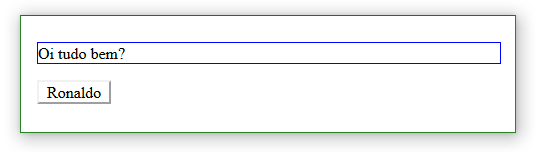
\includegraphics[width=0.5\textwidth]{figuras/jsbase}
\begin{flushleft}
\flushleft{Fonte: Elaborado pelo autor.}
\end{flushleft}
\label{fig:jsbase}
}
\end{figure}

No arquivo~\texttt{app.js}, uma função chamada~\texttt{rename()}~recebe como parâmetro (\texttt{el}) o elemento que a invoca através do evento de~\texttt{onclick=}~do botão. Após isto, o elemento que contém a classe~\texttt{.name} é renomeado para o mesmo texto de dentro do botão (i.e. Ronaldo). Como observado no na linha 9 do Código~\ref{htmlfinal}, dentro do elemento parágrafo~"\texttt{<p>}"~há um texto livre e dentro deste, um elemento~\texttt{<strong>}~com a classe~\texttt{.name}~que receberá o texto do botão. Na Figura~\ref{fig:htmlfinal}~é possível observar o resultado desta interação. É importante ressaltar que o texto recém adicionado como retorno do evento está em negrito por formatação padrão do elemento~\texttt{<strong>}~no navegador em questão e que esta aparência inicial pode ser personalizada com uma folha de estilo.

\begin{figure}[th]
\centering{
\caption{Documento HTML com CSS e JS.}
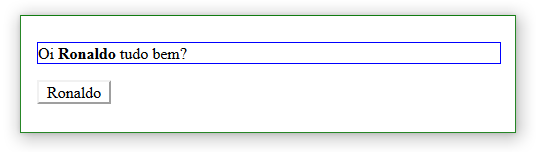
\includegraphics[width=0.5\textwidth]{figuras/htmlfinal}
\begin{flushleft}
\flushleft{Fonte: Elaborado pelo autor.}
\end{flushleft}
\label{fig:htmlfinal}
}
\end{figure}

Além do exemplo apresentado, onde foi realizada uma interação simples na página. É possível com a linguagem JavaScript: Criar validações em formulário, realizar troca de dados com o servidor, computar dados e até gerenciar recursos. Nesta subseção apenas exemplos de JavaScript para \textit{Front-End} foram apresentados, porém, é possível executá-lo no \textit{Back-End}, bem como, Banco de Dados e Sistemas Operacionais também podem ser criados com a linguagem. O grande diferencial da linguagem, além da exclusividade na \textit{Web}, é a comunidade participativa muito responsável pela grande difusão e manutenção de novas soluções com a linguagem.
%
%
%
%
%
%
%
%
%
\section{Elementos Básicos para uma Aplicação \textit{Web} Moderna}
\label{ElementosWeb}

\subsection{AJAX}
\label{SubAJAX}

AJAX significa \textit{Asynchronous JavaScript and XML}, uma técnica para criar aplicações \textit{Web} melhores, mais rápidas e interativas com a ajuda de XML, HTML, CSS e JavaScript. Foi apresentado ao mundo em~\citeonline{garrett2005ajax}, descrevendo a técnica onde dados podem ser carregados em segundo plano sem necessidade de recarga de página. Isso resultou no ressurgimento do JavaScript, sustentado por novas comunidades, bibliotecas e \textit{frameworks}.

Em aplicações \textit{Web} convencionais, o \textit{front-end} transmite informações para o \textit{back-end} utilizando solicitações síncronas. Isso significa, por exemplo, que um formulário é preenchido, o botão de enviar é acionado e há um redirecionamento para uma nova página com novas informações retornadas do servidor. Com o AJAX, quando o formulário é submetido ao servidor, diferentemente do modo síncrono padrão, o JavaScript realiza uma solicitação ao servidor, interpreta os resultados e atualiza a tela atual. No sentido mais puro, o usuário nunca sabe que algo foi transmitido ao servidor.

AJAX é uma tecnologia \textit{Web} independente de software e de servidor, baseada em \textit{Open Standards} (i.e. Padrões Abertos). É comum o uso de XML como formato para o recebimento de dados do servidor, embora qualquer formato, incluindo texto simples, possa ser usado. Utiliza o paradigma \textit{data-driven} em vez de \textit{page-driven}, o que permite que o usuário continue utilizando a aplicação enquanto o AJAX solicita informações do servidor, tudo em segundo plano e assíncrono através de objetos de requisição~\texttt{XMLHttpRequest}, próprios do navegador. AJAX é capaz de realizar requisições em todos os verbos HTTP disponíveis na Subseção~\ref{SubHTTP}~e utiliza JavaScript para fazer tudo.
%
%
%
\subsection{JSON}
\label{SubJSON}

JSON é o acrônimo de \textit{Javascript Object Notation} ou Objeto de Notação JavaScript. É um formato leve de intercâmbio de dados padronizado no RFC 4627 em \citeonline{crockfordrfc}. Para seres humanos, é fácil de ler e escrever, para máquinas, é fácil de interpretar e gerar. Está baseado em um subconjunto da linguagem JavaScript, a notação, origem do nome. JSON é bastante similar ao XML, com a mesma utilidade, mesmo intuito, porém mais leve. Apesar do nome ser bem sugestivo, não necessariamente deve ser utilizado com JavaScript, é um formato de texto e completamente independente de linguagem. Muitas linguagens hoje em dia dão suporte ao JSON, é meio que um novo método, substituto do antigo e conhecido XML. Ele é muito usado para retornar dados vindos de um servidor utilizando requisições AJAX para atualizar dados em tempo real. JSON está constituído em duas estruturas:
\begin{itemize}
    \item Uma coleção de pares nome/valor. Em várias linguagens, isto é caracterizado como um \textit{object}, dicionário, \textit{hash table} ou arrays associativas.
    \item Uma lista ordenada de valores. Na maioria das linguagens, isto é caracterizado como uma \textit{array}, vetor, lista ou sequência.
\end{itemize}

Estas são estruturas de dados universais. Em JSON, os dados são apresentados desta forma: Um objeto é um conjunto desordenado de pares nome/valor. Um objeto começa com uma chave de abertura~"\texttt{\{}"~e termina com uma chave de fechamento~"\texttt{\}}". Cada nome é seguido por dois pontos~"\texttt{:}"~e os pares nome/valor são seguidos por vírgula~"\texttt{,}". Uma \textit{array} é uma coleção de valores ordenados. O \textit{array} começa com colchete de abertura~"\texttt{[}"~e termina com colchete de fechamento~"\texttt{]}". Os valores são separados por vírgula. Por final, um valor pode ser uma cadeia de caracteres, um número, booleano, valor nulo, objeto ou até uma \textit{array}. As estruturas podem estar aninhadas.

\begin{lstlisting}[label=basejson,caption=Exemplo de um arquivo JSON.]
{
  "letras" : [
    { "letra": "A", "numeros": [ { "numero": 5 }, { "numero": 10 } ] },
    { "letra": "B", "numeros": [ { "numero": 7 }, { "numero": 17 } ] },
    { "letra": "C", "numeros": [ { "numero": 9 }, { "numero": 33 } ] }
  ]
}
\end{lstlisting}

Nos códigos~\ref{basexml}~e~\ref{basejson}, é possível observar o quão menor é o arquivo JSON em comparação ao XML, visto que sua estrutura contribui por ser um formato de texto mais simplificado. Os blocos de código contêm, respectivamente para XML e JSON, 509 e 237 caracteres. Uma diminuição de aproximadamente 53\% na quantidade de caracteres necessária para se chegar ao mesmo resultado. Optar pela utilização do JSON em relação ao XML é uma forma de otimização, visto a menor quantidade de dados a serem processados e posteriormente trafegados em rede.

\begin{lstlisting}[label=basexml,caption=Exemplo de um arquivo JSON.]
<?xml version="1.0" encoding="UTF-8"?>
<root>
    <letras>
        <letra>A</letra>
        <numeros>
            <numero>5</numero>
            <numero>10</numero>
        </numeros>
    </letras>
    <letras>
        <letra>B</letra>
        <numeros>
            <numero>7</numero>
            <numero>17</numero>
        </numeros>
    </letras>
    <letras>
        <letra>C</letra>
        <numeros>
            <numero>9</numero>
            <numero>99</numero>
        </numeros>
    </letras>
</root>
\end{lstlisting}
%
%
%
%
%
%
%
%
%
\section{Arquitetura de uma Aplicação}
\label{ArquiteturaWeb}

\subsection{MVC \textit{versus} VMP \textit{versus} MVVM}
\label{SubMVCMVVM}

O principal ponto de partida para decidir qual padrão arquitetural a escolher, é entender suas particularidades e semelhanças, comparando quais as melhores descrições em uma abordagem para o desenvolvimento de software.

Os padrões apresentam objetivos semelhantes, contudo o fazem de maneira distinta e estes objetivos almejam aumentar a modularidade, flexibilidade, testabilidade e manutenibilidade do código. Ainda sobre as semelhanças nas responsabilidades dentro da aplicação, devemos descrevê-las como:
\begin{itemize}
    \item \textit{Model}~\textemdash~Responsável pelo acesso aos dados, contém a lógica necessária para processar estes dados obtidos a fim de retorná-los na forma necessária para que as outras camadas possam utilizá-los.
    \item \textit{View}~\textemdash~Tem todo o desenho e formatação da interface, assim como validações específicas e processa os dados obtidos na UI para disponibilizá-los para as outras camadas.
\end{itemize}

O que diferencia os três padrões de arquitetura no \textit{front-end} é a comunicação entre as camadas e a forma como a terceira camada é organizada e executada. Como observado anteriormente, as camadas \textit{Model} e a \textit{View} são as mesmas para os padrões de arquitetura, distinguindo apenas na terminação dos acrônimos, sendo C, P e VM; Especificadas respectivamente abaixo:
\begin{itemize}
    \item \textit{Controller}~\textemdash~A peça central do MVC que desacopla o \textit{Model} e o \textit{View}. Responsável por toda a lógica de harmonização de dados e as relações entre entidades, bem como o fluxo de eventos por interação do usuário.
    \item \textit{Presenter}~\textemdash~Uma evolução do MVC que torna a arquitetura ainda mais modular desacoplando as funções. A interação com o usuário é feita primariamente na \textit{View} que delegará ao \textit{Presenter} uma tarefa, porém nesta relação, o \textit{Presenter} não pode delegar tarefas para a \textit{View}. Devido ao desacoplamento, testar torna-se mais fácil. É possível vincular dados da \textit{View} com o \textit{Model} através de \textit{data binding}. Isto ocorre na variação \textit{Supervising Controller}, em oposição à variação \textit{Passive View} onde a \textit{View} essencialmente só possui o desenho da UI.
    \item \textit{View-Model}~\textemdash~Diferente dos padrões apresentados anteriormente, este adiciona propriedades e operações ao \textit{Model} para atender as necessidades do \textit{View}, portanto ele cria um novo modelo para a visualização. O \textit{data binding} é feito entre a \textit{View} e o \textit{Model}, criando o \textit{View-Model}. Com esse padrão é possível reduzir a quantidade de código para manter. Algumas automações são possíveis por ter todas as informações necessárias no \textit{View-Model}.
\end{itemize}

Um determinado padrão não necessariamente é melhor que outra arquitetura, o critério de escolha sugerido é a compatibilidade com o projeto. Determinados \textit{frameworks} implementam determinada arquitetura em sua própria estrutura, é recomendável utilizar tal padrão a fim de obter o máximo de desempenho deste \textit{framework} em questão, não existindo assim, uma arquitetura melhor que outra por definitivo.
%
%
%
\subsection{A importância de um serviço \textit{Web}}
\label{SubServicoWeb}
\textit{Web service} (WS) é uma solução utilizada na integração de sistemas e na comunicação entre aplicações diferentes. Com esta tecnologia é possível que novas aplicações possam interagir com aquelas que já existem e que sistemas desenvolvidos em plataformas diferentes sejam compatíveis. Os WS são componentes que permitem às aplicações enviar e receber dados.

As bases para a construção de um WS é o padrão REST ou SOAP. O transporte dos dados é realizado normalmente via protocolo HTTP. Os dados são transferidos em formato de texto. Muitas empresas temiam, no passado, prover funcionalidades na Internet devido ao medo de expor seus dados. Mas com advento dos WS elas podem publicar serviços de forma simples e que são totalmente isolados da base de dados. Os \textit{Web services} permitem que a integração de sistemas seja realizada de forma compreensível, reutilizável e padronizada. É uma tentativa de organizar um cenário cercado por uma grande variedade de diferentes aplicativos, fornecedores e plataformas. Os dois padrões mais comumente utilizados em WS são:
\begin{itemize}
    \item \textbf{SOAP}~\textemdash~Um protocolo de transferência de mensagens em formato XML para uso em ambientes distribuídos. O padrão SOAP funciona como um tipo de \textit{framework} que permite a interoperabilidade entre diversas plataformas com mensagens personalizadas. Aplicando este padrão em \textit{Web Services}, geralmente usa-se o WSDL para descrever a estrutura das mensagens SOAP e as ações possíveis em um \textit{endpoint}. Uma das maiores vantagens disso é que várias linguagens e ferramentas conseguem ler e gerar mensagens facilmente. Várias linguagens de programação permitem a geração de objetos de domínio, \textit{Stubs} e \textit{Skeletons} a partir da definição do WSDL, permitindo a comunicação remota via RPC através de chamadas a métodos remotos, inclusive com argumentos complexos, como se fossem chamadas locais. O problema desse padrão, é que ele adiciona um \textit{overhead} considerável, tanto por ser em XML quanto por adicionar muitas \textit{tags} de meta-informação. Além disso, a serialização e desserialização das mensagens pode consumir um tempo considerável.
    \item \textbf{REST}~\textemdash~Baseado no protocolo de hipermídia HTTP. Porém ele não impõe restrições ao formato da mensagem, apenas no comportamento dos componentes envolvidos. A maior vantagem do protocolo REST é sua flexibilidade. O desenvolvedor pode optar pelo formato mais adequado para as mensagens do sistema de acordo com sua necessidade específica. Os formatos mais comuns são JSON, XML e texto puro, mas em teoria qualquer formato pode ser usado. Isso nos leva a outra vantagem: quase sempre \textit{Web Services} que usam REST são mais "leves" e, portanto, mais rápidos. O problema com o REST pode surgir justamente por causa de suas vantagens. Como a definição do corpo de dados fica totalmente a cargo do desenvolvedor, os problemas de interoperabilidade são mais comuns.
\end{itemize}

Em geral, SOAP é uma boa opção para instituições com padrões rígidos e ambientes complexos. Muitas ferramentas corporativas tiram vantagem do padrão e possibilitam filtrarem, enfileiramento, classificação e redirecionamento das mensagens trocadas entre sistemas. Praticamente todas as plataformas e linguagens modernas suportam esses conceitos e a solução final é muito mais simples do que o equivalente em SOAP. Além disso, integrações com alto volume de requisições são inviáveis em SOAP. REST é capaz de atender volume e complexidade sem dificuldades, exigindo apenas um mínimo de experiência do desenvolvedor para estabelecer e reforçar os padrões adequados.
%
%
%
%
%
%
%
%
%
\section{Ferramentas Avançadas para o Desenvolvimento \textit{Web}}
\label{FerramentasWeb}

Algumas ferramentas e extensões podem ser utilizadas para tornar o desenvolvimento mais ágil. Estes complementos são detalhados na próxima seção, porém, sua escolha é arbitrária e baseada em sua popularidade. Em outras palavras, as ferramentas mais utilizadas pela comunidade de desenvolvedores e que possuem um maior número de contribuidores. Estas ferramentas disponibilizam recursos que agregam mais funcionalidade ao desenvolvimento, tais como: entrada escrita de código de próxima geração e saída de código compatível com os navegadores; verificação de erros sintáticos; \textit{minification} em arquivos; padronização de estilo de código. Estas extensões podem agregar mais funcionalidade para as três tecnologias base, HTML, CSS e JavaScript, renderizadas pelo navegador.